\section*{Radiation Balance Between Parallel Plates}
Assignment is completed by Mikkel Jaedicke (mijae12) \& Anders Bæk (anbae12)


\begin{equation}
\begin{align*}
m_{ 1 }\frac { { d }^{ 2 } }{ { dt }^{ 2 } } \left[ \begin{matrix} x_{ 1 } \\ y_{ 1 } \end{matrix} \right] &=-\frac { m_{ 1 }\cdot M\cdot g }{ { r }^{ 3 }_{ 1 } } \left[ \begin{matrix} x_{ 1 } \\ y_{ 1 } \end{matrix} \right] +\frac { m_{ 1 }\cdot m_2\cdot g }{ { r }^{ 3 }_{ 12 } } \left[ \begin{matrix} x_{ 2 }-x_{ 1 } \\ y_{ 2 }-y_{ 1 } \end{matrix} \right] \\
m_{ 2 }\frac { { d }^{ 2 } }{ { dt }^{ 2 } } \left[ \begin{matrix} x_{ 1 } \\ y_{ 1 } \end{matrix} \right] &=-\frac { m_{ 2 }\cdot M\cdot g }{ { r }^{ 3 }_{ 2 } } \left[ \begin{matrix} x_{ 1 } \\ y_{ 1 } \end{matrix} \right] -\frac { m_{ 1 }\cdot m_{ 2 }\cdot g }{ { r }^{ 3 }_{ 12 } } \left[ \begin{matrix} x_{ 2 }-x_{ 1 } \\ y_{ 2 }-y_{ 1 } \end{matrix} \right] 
\end{align*}
\label{eq:1}
\end{equation}
where: \( m_1 = m_2 =9.20 \cdot 10^{18} \) [kg], \( M = 5.68  \cdot 10^{26} \) [kg], \( g = 4.98 \cdot 10^{-10} \left[ \frac { \text{km}^3 }{ \text{kg} \cdot \text{døgn} }  \right] \).

\begin{equation}
\begin{align*}
\left[ \begin{matrix} x_{ 1 } \\ y_{ 1 } \end{matrix} \right] &=\left[ \begin{matrix} 0 \\ 152870 \end{matrix} \right] ,\frac { d }{ dt } \left[ \begin{matrix} x_{ 1 } \\ y_{ 1 } \end{matrix} \right] =\left[ \begin{matrix} -1360278.1 \\ 0 \end{matrix} \right]  \\
\left[ \begin{matrix} x_{ 2 } \\ y_{ 2 } \end{matrix} \right] &=\left[ \begin{matrix} 0 \\ -153130 \end{matrix} \right] ,\frac { d }{ dt } \left[ \begin{matrix} x_{ 2 } \\ y_{ 2 } \end{matrix} \right] =\left[ \begin{matrix} 1359122.8 \\ 0 \end{matrix} \right] 
\end{align*}
\label{eq:2}
\end{equation}


\begin{figure}[th!]
\centering
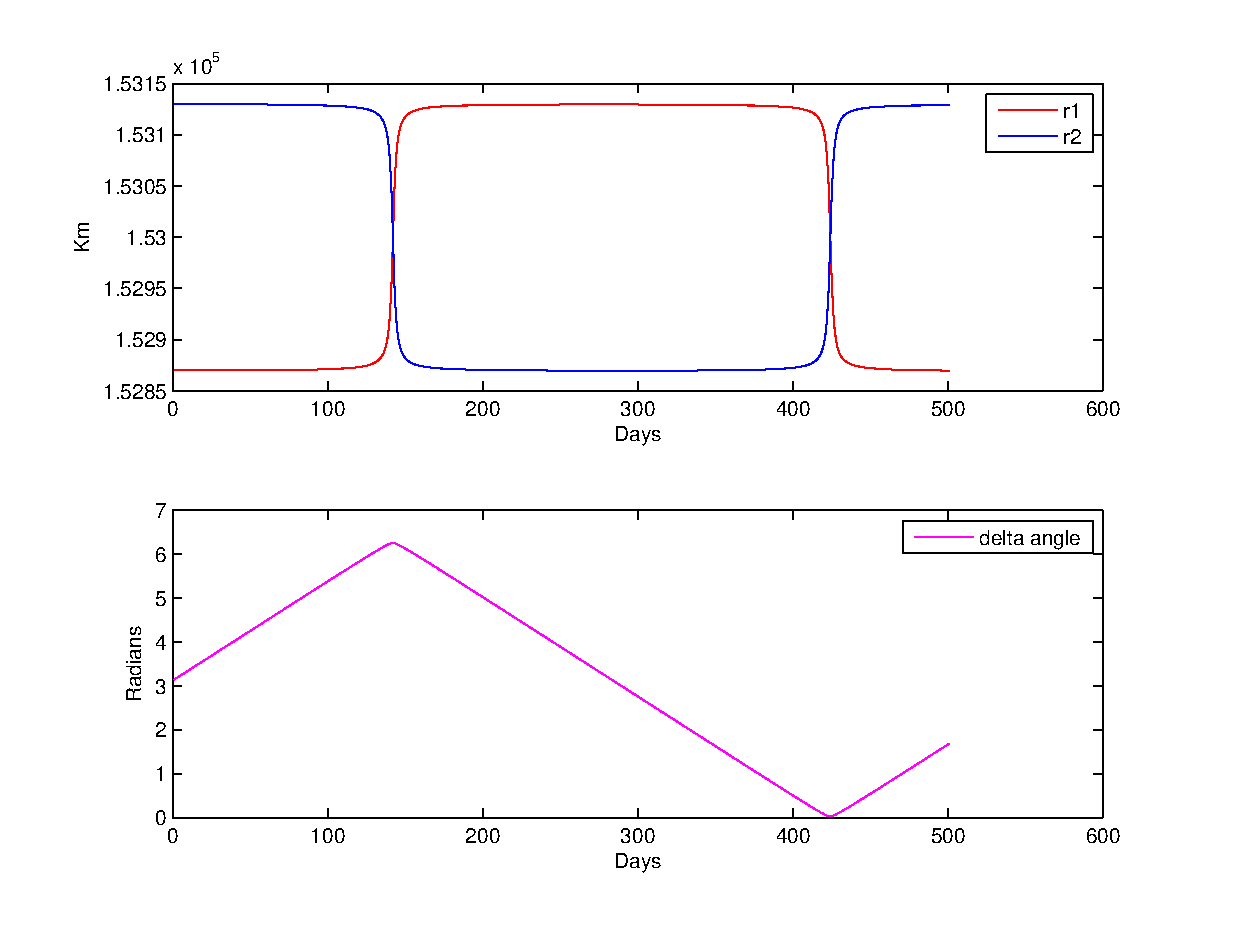
\includegraphics[width=1\textwidth]{./graphics/subplot.eps}
\caption[tekst i indholdsfortegnelsen]{figurtekst}
\label{fig:}
\end{figure}